\chapter{Contexto y estado del técnica}

Después de la introducción, se suele describir el contexto de aplicación. En este Capítulo debemos mostrar un sobrado conocimiento de la materia, plagando absolutamente TODO lo que mencionemos con referencias. Práticamente, cada frase puede necesitar de alguna referencia.

Las referencias NO están solo para aparentar. Rendimos tributo y reconocemos a las personas que han pensado los problemas antes que nosotros. Puede haber varias referencias válidas para una misma afirmación, y no pasa nada porque así se indique.

Recuerda que para citar trabajos de diferentes autores es fundamental e imprescindible seguir el formato APA, según se describe en el documento Normativa\_APA.pdf disponible en el apartado de Documentación del Aula de información general del Máster Universitario en Computación Cuántica (MUCC). No se debe mencionar, ni utilizar ninguna fuente, sin citarla apropiadamente.

EJEMPLO DE CITAS: Si queremos citar a alguien, por ejemplo porque vamos a hablar de Latex \citep{lamport1994} o porque, según las ideas de \cite{ackerman2017}, la liga de fútbol inglesa debe tener torneos de desempate, pues tenemos que hacerlo correctamente. {\bf{(Ver en la sección Bibliografía cómo deben incluirse las entradas bibliográficas).}}

Este Capítulo puede tener secciones diferentes a las que se indican a continuación, que se indican a modo de ejemplo.

\section{Antecedentes históricos}

En 1980, Paul Benioff propone la primera versión teórica de una máquina de Turing cuántica poniendo de manifiesto que la computación cuántica era, en efecto, teóricamente posible (Benioff, 1980). Poco tiempo después, Richard Feynman constató que existían ciertos fenómenos cuya simulación requería de recursos que crecían de manera exponencial con la complejidad del problema y sugirió el empleo de computadores cuánticos para simular este tipo de fenómenos (Feynman, 1982). A mediados de los 80, David Deustch describe la Máquina de Turing Universal Cuántica, probando que construir un computador cuántico era teóricamente posible (Deutsch, 1985). En este mismo artículo, aparece el algoritmo de Deutsch, el primer algoritmo que resuelve un problema de manera más eficiente que su versión clásica.

Durante la década de los 90, aparecerán dos de los algoritmos más importantes en computación cuántica. En primer lugar, el algoritmo de Shor es capaz de factorizar enteros con una ventaja exponencial respecto a los algoritmos clásicos (Shor, 1994). En segundo lugar, el algoritmo de Grover diseñado para realizar búsquedas en una base de datos no estructurada de manera más eficiente (Grover, 1996). La aparición de estos algoritmos pone de manifiesto la existencia de una ventaja cuántica en este nuevo modelo de computación.

Este nuevo paradigma no utiliza bits clásicos  si no bits cuánticos o qubits, término atribuido a Benjamin Schumacher (1995). En el año 2000, Divincenzo propone 5 requisitos que debe cumplir todo sistema para que pueda ser considerado como una implementación física válida de un computador cuántico (Divincenzo, 2000):

\begin{enumerate}
    \item Debe tratarse de un sistema escalable con al menos un qubit bien caracterizado.
    \item Debe poder inicializarse a un estado inicial, habitualmente 
    $ | 0 \rangle $.
    \item Cada qubit debe tener un tiempo de decoherencia significativamente superior a los tiempos de actuación de las puertas cuánticas.
    \item Debe poseer un conjunto universal de puertas cuánticas.
    \item Debe poseer algún mecanismo que permite medir el estado de los qubits.
\end{enumerate}










\section{Estado actual}

En la siguiente sección, se expondrán todos aquellos conceptos de la Mecánica Cuántica y, mas específicamente, de la computación cuántica de los que nos serviremos durante el desarrollo del presente trabajo.

\subsection{Postulados de la mecánica cuántica}

El formalismo matemático de la mecánica cuántica se rige por los siguientes postulados (Nielsen y Chuang, 2010):

\begin{description}
    \item[Postulado 1] Para cada sistema físico, existe un espacio vectorial complejo con producto interno (es decir, un espacio de Hilbert) conocido como espacio de estado. El estado de dicho sistema queda completamente descrito por un vector unitario perteneciente al espacio de estados. 
    
    \item[Postulado 2] El estado de un sistema evoluciona según una transformación unitaria. Es decir, sea el estado $ | \psi \rangle$ y la transformación unitaria definida por el operador unitario $U$, entonces el estado $ | \psi \rangle $ evolucionará al estado $ | \psi' \rangle = U | \psi \rangle$.
    \item[Postulado 3] Las medidas cuánticas están descritas por un conjunto $ \left \{ M_m \right \}  $ de operadores de medida donde los subíndices $m$ hacen referencia al resultado obtenido en cada medida. Si el sistema se encuentra en el estado $ | \psi \rangle $ en el instante inmediatamente anterior a la medida, entonces la probabilidad de obtener el resultado $m$ es $$ p(m)= \langle \psi | M_m^\dagger M_m | \psi \rangle $$ y el estado del sistema tras la medida será $$ \frac{M_m | \psi \rangle}{\sqrt{\langle \psi | M_m^\dagger M_m | \psi \rangle}} . $$
    \item[Postulado 4] El espacio de estados correspondiente a un sistema físico compuesto viene dado por el producto tensorial de los espacios de estados correspondientes a cada uno de los sistemas físicos que componen nuestro sistema, es decir, $$| \psi \rangle = | \psi_1 \rangle \otimes | \psi_2 \rangle \otimes ... \otimes | \psi_n \rangle .$$
\end{description}

\subsection{Qubit}

Matemáticamente, un qubit es un vector unitario perteneciente a un espacio vectorial complejo de dimensión 2 para el cual existe una base ortonormal determinada por $ \left \{ | 0 \rangle , | 1 \rangle  \right \}$ (Rieffel y Polak, 2000). Así pues, el estado de un qubit queda determinado por cualquier combinación lineal $ | \psi \rangle = \alpha | 0 \rangle + \beta | 1 \rangle $ donde $ \alpha, \beta \in \mathbb{C} $ tal que $ | \alpha |^2 + | \beta |^2=1 $.

Los vectores que forman la base $\{ |0 \rangle , |1 \rangle  \}$ vienen dados por

$$ |0 \rangle = \begin{pmatrix} 1\\ 0 \end{pmatrix}, |1 \rangle = \begin{pmatrix} 0\\ 1 \end{pmatrix}.$$

Existen ciertos estados que, debido a su recurrencia, poseen una denotación propia (Nielsen y Chuang, 2010). Estos estados son los siguientes:

$$ | + \rangle = \frac{1}{\sqrt{2}} | 0 \rangle + \frac{1}{\sqrt{2}} | 1 \rangle $$
$$ | - \rangle = \frac{1}{\sqrt{2}} | 0 \rangle - \frac{1}{\sqrt{2}} | 1 \rangle $$
$$ | i \rangle = \frac{1}{\sqrt{2}} | 0 \rangle + \frac{i}{\sqrt{2}} | 1 \rangle $$
$$ | -i \rangle = \frac{1}{\sqrt{2}} | 0 \rangle - \frac{i}{\sqrt{2}} | 1 \rangle $$

Ya que $ \langle \psi | \psi \rangle = | \alpha |^2 + | \beta |^2=1$, entonces existe $ \theta \in [0, \pi]$ tal que $ | \alpha | = cos ( \frac{\theta}{2} )$ y $ | \beta | = sen ( \frac{\theta}{2} )$. De este modo, el estado de un qubit se puede representar de la siguiente manera

$$ | \psi \rangle = cos ( \frac{\theta}{2}) | 0 \rangle + e^{i \phi} sen ( \frac{\theta}{2} ) | 1 \rangle  $$

donde $\phi \in [0 , 2 \pi)$ representa la fase relativa entre los coeficientes (Willsh, Willsh y Michielsen, 2022).

De la expresión anterior, se sigue que existe una aplicación biyectiva entre cada estado cuántico y la superficie de una esfera tridimensional de radio 1, es decir, el estado cuántico de un qubit puede representarse como un punto sobre la superficie de una esfera de radio igual a 1. Esta representación se conoce como representación sobre la esfera de Bloch (1946).



\begin{figure}[ht]
	\begin{center}
		\caption{Representación sobre la Esfera de Bloch}
		\label{fig:fig-1}
		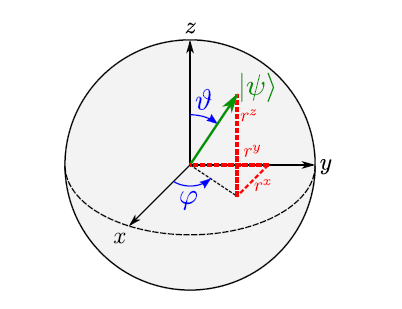
\includegraphics[width=0.5\linewidth]{Bloch.PNG}
		\small Fuente: American Psychological Association, 2020f.
	\end{center}
\end{figure}

\subsection{Medida}

En virtud del postulado 3 de la Mecánica Cuántica, existen dos resultados posibles cuando medimos el estado de un qubit, $ |0 \rangle $ o $ | 1 \rangle$. Sea el estado $ | \psi \rangle = \alpha | 0 \rangle + \beta | 1 \rangle$, entonces como resultado de una medición se obtendrá el estado $| 0 \rangle$ con una probabilidad $ | \alpha|^2$ y el estado $ | 1 \rangle $ con una probabilidad $ | \beta |^2$.

Una importante característica de las medidas cuánticas es que el estado inmediatamente anterior a la medida es destruido y sustituido por el resultado obtenido en la medida. Veamos qué implicaciones tiene esto para la cantidad de información que puede codificarse sobre un único qubit.

Como hemos visto anteriormente, cada estado cuántico se corresponde con un único punto sobre la esfera de Bloch. Dado que la superficie de la esfera tiene infinitos puntos cabría esperar que, en principio, cualquier cantidad de información pudiera ser codificada en un único qubit. No obstante, es necesario prestar atención a la naturaleza intrínseca de las medidas cuánticas ya que solo dos resultados posibles pueden producirse. Dicho de otro modo, de un único qubit mediante una medida, únicamente puede obtenerse un bit de información clásica de su estado (Nielsen y Chuang, 2010).

Otra cuestión interesante respecto a las medidas cuánticas es que pueden realizarse respecto a cualquier a base ortonormal del espacio de Hilbert. Por ejemplo, si se mide un qubit respecto de la base $\{ |+ \rangle, | - \rangle \}$, conocida como base de Hadamard, entonces los posibles resultados serán los estados $ | + \rangle$ y $ | - \rangle $. De esto, se deduce que la superposición cuántica es un fenómeno relativo a la base utilizada. Es decir, si se mide el estado $| + \rangle $ respecto de la base computacional $\{ |0 \rangle, | 1 \rangle \}$, se obtendrá el estado $ | 0 \rangle $ con un 50 $ \% $ de probabilidad o el estado $ | 1 \rangle $ con otro 50 $ \% $ de probabilidad. Queda claro que el estado $ | + \rangle $ encarna una superposición uniforme respecto de la base computacional. Del mismo modo, si se mide el estado $| 1 \rangle $ respecto de la base de Hadamard $\{ |+ \rangle, | - \rangle \}$, se obtendrá el estado $ | + \rangle $ con un 50 $ \% $ de probabilidad o el estado $ | - \rangle $ con otro 50 $ \% $ de probabilidad. Se deduce que el estado $ | 1 \rangle $ presenta una superposición uniforme respecto de la base Hadamard.

